%% =======================================================
%% Actividad 5: Visualizaciones para clasificación
%%
%% Compilar desde actividades/: ./compilar.sh act05
%% Las figuras de img/ se generan con: python act05.py
%% =======================================================

%% ---- CONFIGURACIÓN ------------------------

\documentclass[11pt,letterpaper]{article}

\usepackage[indice]{tecnm}
\usepackage[T1]{fontenc}
\usepackage{amsmath}
\usepackage{xcolor}
\usepackage[most]{tcolorbox} % Carga tcolorbox con soporte para listings y saltos de página
\tcbuselibrary{listings, skins, breakable}
\setlength{\emergencystretch}{3em} % Evita líneas desbordadas por palabras en \texttt

% Paleta de colores (estilo GitHub Light / VS Code)
\definecolor{codebg}{HTML}{F8F9FA}       % Fondo del código
\definecolor{codehead}{HTML}{E9ECEF}     % Fondo de la barra de título
\definecolor{codeborder}{HTML}{CED4DA}   % Borde de la tarjeta
\definecolor{codetitle}{HTML}{212529}    % Texto del título
\definecolor{codekw}{HTML}{0550AE}       % Palabras clave (import, def, for...)
\definecolor{codefunc}{HTML}{8250DF}     % Funciones y métodos (describe, groupby...)
\definecolor{codestr}{HTML}{0A3069}      % Strings
\definecolor{codecomm}{HTML}{6E7781}     % Comentarios
\definecolor{codenum}{HTML}{8C959F}      % Números de línea
\definecolor{codeid}{HTML}{24292F}       % Texto general

% Configuración base de listings
\lstdefinestyle{pythonestilo}{
  language=Python,
  basicstyle=\ttfamily\footnotesize\color{codeid},
  keywordstyle=\color{codekw}\bfseries,
  keywordstyle=[2]\color{codefunc}, % Estilo secundario para métodos de datos
  stringstyle=\color{teal!80!black},
  commentstyle=\color{codecomm}\itshape,
  morekeywords={as, True, False, None, with, yield, lambda},
  morekeywords=[2]{describe, value_counts, print, len, DataFrame, Series, boxplot, boxplot_stats, hist, scatter, plot, axvline, axvspan, axhline, polyfit, corrcoef, linspace, subplots, figure, savefig, tight_layout, concatenate, clip, normal, uniform, randint, seed, mean, median, std, cut, round},
  numbers=left,
  numberstyle=\tiny\ttfamily\color{codenum},
  stepnumber=1,
  numbersep=10pt,
  showstringspaces=false,
  morestring=[b]{"""},
  tabsize=4,
  breaklines=true,
  breakatwhitespace=true,
  columns=flexible,
  keepspaces=true,
  literate=
    {á}{{\'a}}1 {é}{{\'e}}1 {í}{{\'i}}1 {ó}{{\'o}}1 {ú}{{\'u}}1
    {Á}{{\'A}}1 {É}{{\'E}}1 {Í}{{\'I}}1 {Ó}{{\'O}}1 {Ú}{{\'U}}1
    {ñ}{{\~n}}1 {Ñ}{{\~N}}1 {¿}{{?`}}1 {¡}{{!`}}1
}

% Definición del entorno personalizado \begin{codigo}{Título}{etiqueta}
% \newtcblisting[auto counter, number within=section]{codigo}[2][]{
\newtcblisting[auto counter]{codigo}[2][]{
  listing only,
  breakable,                    % Permite que el bloque se divida si pasa de página
  enhanced,
  colback=codebg,
  colframe=codeborder,
  colbacktitle=codehead,
  coltitle=codetitle,
  fonttitle=\bfseries\small\sffamily,
  boxrule=0.6pt,
  arc=4pt,                      % Bordes redondeados
  left=20pt,                    % Espacio izquierdo para los números de línea
  right=8pt,
  top=6pt,
  bottom=6pt,
  toptitle=4pt,
  bottomtitle=4pt,
  before skip=12pt,
  after skip=12pt,
  listing options={style=pythonestilo},
  title={Código \thetcbcounter: #2},
  #1
}

% Paleta para salida de consola (estilo terminal limpia)
\definecolor{termbg}{HTML}{212529}      % Fondo oscuro tipo terminal
\definecolor{termhead}{HTML}{343A40}    % Barra superior
\definecolor{termtext}{HTML}{F8F9FA}    % Texto claro de alta legibilidad
\definecolor{termborder}{HTML}{495057}  % Borde

% Entorno \begin{consola}[label=out:iris]{Título}
\newtcblisting[auto counter]{consola}[2][]{
  listing only,
  breakable,
  colback=termbg,
  colframe=termborder,
  colbacktitle=termhead,
  coltitle=termtext,
  colupper=termtext,
  fonttitle=\bfseries\small\sffamily,
  boxrule=0.6pt,
  arc=4pt,
  left=8pt,
  right=8pt,
  top=6pt,
  bottom=6pt,
  toptitle=4pt,
  bottomtitle=4pt,
  before skip=12pt,
  after skip=12pt,
  listing options={
    basicstyle=\ttfamily\scriptsize\color{termtext}, % \scriptsize evita que las tablas de Pandas se partan de línea
    breaklines=true,
    columns=fixed,        % Mantiene alineadas las columnas de Pandas
    keepspaces=true,
    showstringspaces=false,
    literate=
      {á}{{\'a}}1 {é}{{\'e}}1 {í}{{\'i}}1 {ó}{{\'o}}1 {ú}{{\'u}}1
      {Á}{{\'A}}1 {É}{{\'E}}1 {Í}{{\'I}}1 {Ó}{{\'O}}1 {Ú}{{\'U}}1
      {ñ}{{\~n}}1 {Ñ}{{\~N}}1
  },
  title={Salida \thetcbcounter: #2},
  #1
}

%% ---- DATOS DE LA MATERIA ------------------------

\materia{Modelos Estadísticos para el Aprendizaje \\ Automático y Ciencia de Datos}
\actividad{Tema 1.4
Visualizaciones para Clasificación \\ Actividad 5 - Boxplots, Histogramas y Diagramas de Dispersión}

\profesor{Dr. José Ismael Ojeda Campaña}
%\fecha{15 de octubre de 2026}    % opcional; por defecto es la fecha de hoy

\begin{document}
\portada
\indicegeneral

%% ---- CONTENIDO ---------------------------------

\section{Introducción}

En un problema de clasificación, antes de entrenar cualquier modelo conviene entender cómo se comportan las variables respecto a las clases o grupos de interés. Las visualizaciones son parte fundamental de este análisis exploratorio, porque permiten identificar patrones, relaciones y posibles inconvenientes en los datos antes de implementar modelos de predicción \parencite{tecnm2026_documento_fuente,brownlee2019}.

En este documento se resuelven los seis ejercicios prácticos del tema 1.4, organizados en tres tipos de gráficos: diagramas de caja, histogramas y diagramas de dispersión por clase. Cada ejercicio parte del código base de solución incluido en el documento fuente, que simula los datos del enunciado y genera la gráfica con \texttt{matplotlib}. El código base se extendió con elementos visuales y resúmenes numéricos que permiten interpretar cada gráfica con mayor precisión: medias, cuartiles, detección de valores atípicos, tablas de frecuencias, rectas de regresión y coeficientes de correlación.

\section{Marco conceptual}

\subsection{Visualización en problemas de clasificación}

La visualización facilita estudiar el comportamiento de las variables con respecto a las clases objetivo. En clasificación, la idea central es comparar cómo se distribuye una característica en cada clase. Si las distribuciones son muy distintas entre clases, la característica será útil para separarlas; si se superponen, aportará poca información a un modelo \parencite{tecnm2026_documento_fuente}. Los tres gráficos de este tema ofrecen perspectivas complementarias sobre esa separabilidad.

\subsection{Diagramas de caja}

El diagrama de caja y bigotes (\textit{boxplot}) muestra cómo se distribuye una variable continua a partir de la mediana, los cuartiles y los valores atípicos. No requiere que la distribución sea normal y ofrece una visión clara de la variabilidad \parencite{tecnm2026_documento_fuente,brownlee2019}. Sus elementos son \parencite{tecnm2026_documento_fuente,bruce2020}:

\begin{itemize}
    \item \textbf{Caja:} abarca desde el primer cuartil ($Q_1$) hasta el tercero ($Q_3$), es decir, el 50\,\% central de los datos. Su altura es el rango intercuartílico, $\text{RIC} = Q_3 - Q_1$.
    \item \textbf{Línea dentro de la caja:} la mediana.
    \item \textbf{Bigotes:} muestran la extensión de los datos sin incluir los valores atípicos. En \texttt{matplotlib} llegan, por omisión, hasta el dato más extremo que no se aleja más de $1.5\,\text{RIC}$ de la caja.
    \item \textbf{Valores atípicos:} los puntos más allá de los bigotes, es decir, menores que $Q_1 - 1.5\,\text{RIC}$ o mayores que $Q_3 + 1.5\,\text{RIC}$.
\end{itemize}

En clasificación se dibuja una caja por categoría para determinar si la variable se distribuye de forma diferente en cada clase \parencite{tecnm2026_documento_fuente}.

\subsection{Histogramas}

El histograma divide los datos en intervalos (\textit{bins}) y representa la frecuencia de valores en cada uno. Muestra la forma de la distribución y puede revelar patrones como asimetría o multimodalidad \parencite{tecnm2026_documento_fuente,brownlee2019}. La forma se relaciona con la posición de la media y la mediana \parencite{tecnm2026_documento_fuente}:

\begin{itemize}
    \item En una distribución \textbf{simétrica}, la media y la mediana coinciden.
    \item En una distribución \textbf{sesgada a la derecha} (sesgo positivo), la cola se extiende hacia los valores altos y la media es mayor que la mediana.
    \item En una distribución \textbf{sesgada a la izquierda} (sesgo negativo), la cola se extiende hacia los valores bajos y la media es menor que la mediana.
\end{itemize}

\subsection{Diagramas de dispersión por clase}

El diagrama de dispersión muestra la relación entre dos variables. Cuando los puntos se colorean según su categoría, se vuelve una herramienta efectiva para explorar la separabilidad visual entre clases y para decidir si una combinación de características es útil para un modelo de clasificación \parencite{tecnm2026_documento_fuente,brownlee2019}. Al diagrama puede agregarse una recta de regresión, que ayuda a visualizar la tendencia general y la correlación lineal entre las variables \parencite{tecnm2026_documento_fuente}. La fuerza de esa relación lineal se mide con el coeficiente de correlación de Pearson, $r$, que va de $-1$ a $1$: valores cercanos a $\pm 1$ indican una relación lineal fuerte y valores cercanos a 0, ausencia de relación lineal \parencite{bruce2020}.

\section{Descripción de la actividad}

\textbf{Objetivo:} Elaborar e interpretar diagramas de caja, histogramas y diagramas de dispersión por clase a partir de datos simulados, para comparar la distribución de una variable entre grupos y analizar la relación entre variables.

Los ejercicios del cuaderno de trabajo son los siguientes \parencite{tecnm2026_documento_fuente}:

\begin{description}
    \item[Boxplots, Ejercicio 1.] Comparar mediante un diagrama de caja la mediana, la dispersión y los posibles valores atípicos de las calificaciones finales de 30 estudiantes del Grupo A y 30 del Grupo B.
    \item[Boxplots, Ejercicio 2.] Comparar mediante un diagrama de caja la dispersión, la mediana y los valores atípicos de los tiempos de espera (en minutos) de 40 clientes en cada una de tres sucursales.
    \item[Histogramas, Ejercicio 1.] Simular los tiempos de entrega de 200 pedidos, donde la mayoría se entrega entre 2 y 7 días pero algunos tardan hasta 15, elaborar su histograma y comentar qué información se obtiene.
    \item[Histogramas, Ejercicio 2.] Simular las calificaciones de 120 estudiantes en un examen de matemáticas, la mayoría entre 60 y 90 con algunos casos muy bajos o muy altos, elaborar su histograma y analizar las conclusiones que se pueden extraer.
    \item[Dispersión, Ejercicio 1.] Elaborar un diagrama de dispersión entre las horas de estudio semanales y la calificación final de 25 estudiantes de cada turno (matutino y vespertino), con un color por turno, y analizarlo.
    \item[Dispersión, Ejercicio 2.] Simular la edad y el nivel de colesterol de 40 pacientes clasificados según su actividad física (baja o alta), elaborar el diagrama de dispersión con un color por grupo y comentar los patrones observados.
\end{description}

\section{Desarrollo}

Los seis ejercicios se resolvieron en un solo script, \texttt{act05.py}. Para cada uno se tomó el código base de solución del documento fuente, conservando su semilla aleatoria, su simulación de datos y su gráfica, y se le agregaron las siguientes extensiones:

\begin{itemize}
    \item \textbf{Figuras guardadas como archivo.} Cada gráfica se guarda como imagen PNG en la carpeta \texttt{img/} mediante la función \texttt{guardar()}, de modo que las figuras se incluyen directamente en este reporte. Cuando el código se ejecuta como script, las figuras no se abren en pantalla y el script corre completo de una vez; cuando se ejecuta en un cuaderno como Colab, además se muestran con \texttt{plt.show()}.
    \item \textbf{Resumen numérico de los diagramas de caja.} La función \texttt{resumen\_boxplot()} usa \texttt{boxplot\_stats()} de \texttt{matplotlib} para obtener exactamente los valores que dibuja cada caja (cuartiles, RIC, bigotes y valores atípicos), junto con la media y la desviación estándar.
    \item \textbf{Observaciones individuales.} La función \texttt{puntos\_dispersos()} dibuja cada dato sobre su caja con un pequeño desplazamiento horizontal aleatorio, para que se aprecie cuántos datos hay y cómo se reparten.
    \item \textbf{Medidas de tendencia central.} Los diagramas de caja marcan la media con un rombo rojo y los histogramas la muestran como línea vertical junto a la mediana.
    \item \textbf{Regresión y correlación.} En los diagramas de dispersión se calculan, por grupo, la recta de mínimos cuadrados con \texttt{np.polyfit()} y el coeficiente de correlación de Pearson con \texttt{np.corrcoef()}.
\end{itemize}

En la versión 3.9 de \texttt{matplotlib}, el parámetro \texttt{labels} de \texttt{boxplot()} que usa el código base cambió de nombre a \texttt{tick\_labels}, por lo que se actualizó para evitar la advertencia de obsolescencia. El Código~\ref{cod:comun} contiene las importaciones y funciones auxiliares. El cuaderno interactivo puede consultarse en Google Colab:

\begin{center}
    \url{https://colab.research.google.com/drive/1gfTBEYJqgr0WmeH6V-_5dA9kmYknI49b?usp=sharing}
\end{center}

\begin{codigo}[label=cod:comun]{Importaciones y funciones auxiliares}
import os

import matplotlib

# En Colab o Jupyter no existe __file__; ahí las figuras también se muestran en pantalla
EN_NOTEBOOK = '__file__' not in globals()
if not EN_NOTEBOOK:
    matplotlib.use('Agg')  # Como script, genera las figuras como archivos PNG sin abrir ventanas

import matplotlib.pyplot as plt
import numpy as np
import pandas as pd
from matplotlib.cbook import boxplot_stats

# Carpeta donde se guardan las figuras que se incluyen en el reporte
BASE = os.getcwd() if EN_NOTEBOOK else os.path.dirname(os.path.abspath(__file__))
CARPETA_IMG = os.path.join(BASE, 'img')
os.makedirs(CARPETA_IMG, exist_ok=True)


def guardar(nombre):
    """Guarda la figura actual en la carpeta img/ y la muestra si se ejecuta en un notebook."""
    plt.tight_layout()
    plt.savefig(os.path.join(CARPETA_IMG, nombre), dpi=150)
    if EN_NOTEBOOK:
        plt.show()
    plt.close()


def resumen_boxplot(grupos):
    """Calcula lo que dibuja cada caja: cuartiles, bigotes y valores atípicos."""
    filas = {}
    for nombre, datos in grupos.items():
        s = boxplot_stats(datos)[0]
        filas[nombre] = {
            'Q1': s['q1'], 'Mediana': s['med'], 'Q3': s['q3'], 'RIC': s['iqr'],
            'Bigote inf.': s['whislo'], 'Bigote sup.': s['whishi'],
            'Media': s['mean'], 'Desv. est.': np.std(datos, ddof=1),
            'Atípicos': len(s['fliers']),
        }
    # Una columna por grupo para que la tabla quepa en la consola
    return pd.DataFrame(filas).round(2)


def puntos_dispersos(ax, grupos, semilla=0):
    """Dibuja cada observación sobre su caja con un pequeño desplazamiento horizontal."""
    rng = np.random.default_rng(semilla)
    for i, datos in enumerate(grupos, start=1):
        x = i + rng.uniform(-0.12, 0.12, len(datos))
        ax.scatter(x, datos, s=12, color='black', alpha=0.4, zorder=3)


def correlacion(x, y):
    return np.corrcoef(x, y)[0, 1]
\end{codigo}

\subsection{Diagramas de caja}

\begin{codigo}[label=cod:box1]{Boxplots, Ejercicio 1: calificaciones de dos grupos}
# Código base del documento fuente
np.random.seed(10)
calificaciones_grupo_A = np.random.randint(60, 100, 30)
calificaciones_grupo_B = np.random.randint(50, 95, 30)

# Extensión: medias, observaciones individuales y resumen numérico
fig, ax = plt.subplots(figsize=(7, 5))
ax.boxplot([calificaciones_grupo_A, calificaciones_grupo_B],
           tick_labels=['Grupo A', 'Grupo B'],
           patch_artist=True, showmeans=True,
           boxprops=dict(facecolor='lightblue'),
           meanprops=dict(marker='D', markerfacecolor='red', markeredgecolor='red'))
puntos_dispersos(ax, [calificaciones_grupo_A, calificaciones_grupo_B])
ax.set_title('Comparación de calificaciones finales entre dos grupos')
ax.set_ylabel('Calificación')
ax.grid(axis='y', linestyle='--', alpha=0.7)
guardar('boxplot_ej1.png')

print("=== Boxplots - Ejercicio 1: calificaciones por grupo ===")
print(resumen_boxplot({'Grupo A': calificaciones_grupo_A,
                       'Grupo B': calificaciones_grupo_B}))
\end{codigo}

\begin{codigo}[label=cod:box2]{Boxplots, Ejercicio 2: tiempos de espera en tres sucursales}
# Código base del documento fuente
np.random.seed(20)
tiempos_sucursal_1 = np.random.normal(15, 3, 40)
tiempos_sucursal_2 = np.random.normal(20, 5, 40)
tiempos_sucursal_3 = np.random.normal(10, 2, 40)
tiempos = [tiempos_sucursal_1, tiempos_sucursal_2, tiempos_sucursal_3]
sucursales = ['Sucursal 1', 'Sucursal 2', 'Sucursal 3']

# Extensión: un color por sucursal, medias y observaciones individuales
fig, ax = plt.subplots(figsize=(7, 5))
cajas = ax.boxplot(tiempos, tick_labels=sucursales, patch_artist=True, showmeans=True,
                   meanprops=dict(marker='D', markerfacecolor='red', markeredgecolor='red'))
for caja, color in zip(cajas['boxes'], ['skyblue', 'lightgreen', 'lightcoral']):
    caja.set_facecolor(color)
puntos_dispersos(ax, tiempos)
ax.set_title('Comparación de tiempos de espera en tres sucursales')
ax.set_ylabel('Tiempo de espera (minutos)')
ax.grid(axis='y', linestyle='--', alpha=0.7)
guardar('boxplot_ej2.png')

print("\n=== Boxplots - Ejercicio 2: tiempos de espera por sucursal ===")
resumen = resumen_boxplot(dict(zip(sucursales, tiempos)))
print(resumen)
for nombre, datos in zip(sucursales, tiempos):
    atipicos = boxplot_stats(datos)[0]['fliers']
    if len(atipicos):
        print(f"Valores atípicos en {nombre}: {np.round(atipicos, 2).tolist()}")
\end{codigo}

\subsection{Histogramas}

En el Ejercicio 1 se sombreó la zona de retraso (más de 7 días) y se calculó qué porcentaje de pedidos cae en ella. En el Ejercicio 2 se construyó una tabla de frecuencias por rangos de calificación con \texttt{pd.cut()}.

\begin{codigo}[label=cod:hist1]{Histogramas, Ejercicio 1: tiempos de entrega de 200 pedidos}
# Código base del documento fuente
np.random.seed(100)
tiempos_entrega = np.concatenate([
    np.random.normal(4, 1, 180),   # mayoría de los pedidos
    np.random.uniform(8, 15, 20)   # algunos retrasados
])
tiempos_entrega = np.clip(tiempos_entrega, 1, 15)  # limitar entre 1 y 15 días

# Extensión: media, mediana y zona de retraso (más de 7 días)
media, mediana = tiempos_entrega.mean(), np.median(tiempos_entrega)
plt.figure(figsize=(8, 5))
plt.hist(tiempos_entrega, bins=14, color='skyblue', edgecolor='black')
plt.axvspan(7, 15, color='red', alpha=0.08, label='Retraso (> 7 días)')
plt.axvline(media, color='red', linestyle='--', linewidth=2, label=f'Media: {media:.2f}')
plt.axvline(mediana, color='green', linestyle='-', linewidth=2, label=f'Mediana: {mediana:.2f}')
plt.title('Distribución de tiempos de entrega de pedidos')
plt.xlabel('Tiempo de entrega (días)')
plt.ylabel('Número de pedidos')
plt.grid(axis='y', linestyle='--', alpha=0.7)
plt.legend()
guardar('histograma_ej1.png')

retrasados = tiempos_entrega > 7
print("\n=== Histogramas - Ejercicio 1: tiempos de entrega ===")
print(pd.Series(tiempos_entrega).describe().round(2).to_string())
print(f"Mediana: {mediana:.2f} días")
print(f"Pedidos entregados entre 2 y 7 días: "
      f"{((tiempos_entrega >= 2) & (tiempos_entrega <= 7)).mean():.1%}")
print(f"Pedidos con más de 7 días: {retrasados.sum()} ({retrasados.mean():.1%})")
\end{codigo}

\begin{codigo}[label=cod:hist2]{Histogramas, Ejercicio 2: calificaciones de 120 estudiantes}
# Código base del documento fuente
np.random.seed(200)
calificaciones = np.concatenate([
    np.random.normal(75, 8, 110),   # mayoría de los estudiantes
    np.random.uniform(30, 59, 5),   # calificaciones bajas
    np.random.uniform(91, 100, 5)   # calificaciones altas
])
calificaciones = np.clip(calificaciones, 0, 100)

# Extensión: media, mediana y tabla de frecuencias por rango de calificación
media, mediana = calificaciones.mean(), np.median(calificaciones)
plt.figure(figsize=(8, 5))
plt.hist(calificaciones, bins=10, color='orange', edgecolor='black')
plt.axvline(media, color='red', linestyle='--', linewidth=2, label=f'Media: {media:.2f}')
plt.axvline(mediana, color='green', linestyle='-', linewidth=2, label=f'Mediana: {mediana:.2f}')
plt.title('Distribución de calificaciones en el examen final')
plt.xlabel('Calificación')
plt.ylabel('Número de estudiantes')
plt.grid(axis='y', linestyle='--', alpha=0.7)
plt.legend()
guardar('histograma_ej2.png')

rangos = pd.cut(calificaciones, bins=[0, 60, 70, 80, 90, 100],
                labels=['< 60', '60-70', '70-80', '80-90', '> 90'], include_lowest=True)
tabla = pd.Series(rangos).value_counts(sort=False).to_frame('Estudiantes')
tabla['Porcentaje'] = (tabla['Estudiantes'] / len(calificaciones) * 100).round(1)
tabla.index.name = 'Rango'

print("\n=== Histogramas - Ejercicio 2: calificaciones ===")
print(pd.Series(calificaciones).describe().round(2).to_string())
print(f"Mediana: {mediana:.2f}")
print(tabla)
\end{codigo}

\subsection{Diagramas de dispersión}

En ambos ejercicios los datos de cada grupo se guardan en un diccionario, lo que permite dibujar los puntos y calcular sus estadísticas con un mismo ciclo. El valor de $r$ de cada grupo se agrega a la leyenda de la gráfica.

\begin{codigo}[label=cod:disp1]{Dispersión, Ejercicio 1: horas de estudio vs. calificación por turno}
# Código base del documento fuente
np.random.seed(123)
horas_matutino = np.random.normal(8, 2, 25)
calif_matutino = horas_matutino * 6 + np.random.normal(40, 5, 25)
horas_vespertino = np.random.normal(6, 2, 25)
calif_vespertino = horas_vespertino * 7 + np.random.normal(38, 7, 25)

turnos = {
    'Matutino': (horas_matutino, calif_matutino, 'blue'),
    'Vespertino': (horas_vespertino, calif_vespertino, 'green'),
}

# Extensión: recta de regresión y coeficiente de correlación por turno
plt.figure(figsize=(8, 5))
filas = {}
for turno, (x, y, color) in turnos.items():
    pendiente, ordenada = np.polyfit(x, y, 1)
    r = correlacion(x, y)
    plt.scatter(x, y, color=color, label=f'{turno} (r = {r:.2f})', alpha=0.7)
    xs = np.linspace(x.min(), x.max(), 50)
    plt.plot(xs, pendiente * xs + ordenada, color=color, linewidth=2)
    filas[turno] = {'Horas (media)': x.mean(), 'Calificación (media)': y.mean(),
                    'Pendiente': pendiente, 'Ordenada': ordenada, 'r de Pearson': r}
plt.title('Horas de estudio vs. calificación por turno escolar')
plt.xlabel('Horas de estudio semanales')
plt.ylabel('Calificación final')
plt.legend()
plt.grid(True, linestyle='--', alpha=0.6)
guardar('dispersion_ej1.png')

print("\n=== Dispersión - Ejercicio 1: horas de estudio vs. calificación ===")
print(pd.DataFrame(filas).round(2))
# La simulación del código base no limita la calificación a 100
for turno, (x, y, color) in turnos.items():
    print(f"Calificaciones mayores a 100 ({turno}): {(y > 100).sum()}")
\end{codigo}

\begin{codigo}[label=cod:disp2]{Dispersión, Ejercicio 2: edad vs. colesterol por actividad física}
# Código base del documento fuente
np.random.seed(321)
edad_bajo = np.random.randint(30, 60, 20)
colesterol_bajo = np.random.normal(220, 20, 20)
edad_alto = np.random.randint(30, 60, 20)
colesterol_alto = np.random.normal(190, 15, 20)

grupos = {
    'Actividad física baja': (edad_bajo, colesterol_bajo, 'red'),
    'Actividad física alta': (edad_alto, colesterol_alto, 'purple'),
}

# Extensión: colesterol medio de cada grupo y correlación edad-colesterol
plt.figure(figsize=(8, 5))
filas = {}
for grupo, (x, y, color) in grupos.items():
    r = correlacion(x, y)
    plt.scatter(x, y, color=color, label=f'{grupo} (r = {r:.2f})', alpha=0.7)
    plt.axhline(y.mean(), color=color, linestyle='--', linewidth=1.5)
    filas[grupo] = {'Edad (media)': x.mean(), 'Colesterol (media)': y.mean(),
                    'Colesterol (desv. est.)': np.std(y, ddof=1), 'r de Pearson': r}
plt.title('Edad vs. nivel de colesterol por grupo de actividad física')
plt.xlabel('Edad (años)')
plt.ylabel('Colesterol (mg/dL)')
plt.legend()
plt.grid(True, linestyle='--', alpha=0.6)
guardar('dispersion_ej2.png')

print("\n=== Dispersión - Ejercicio 2: edad vs. colesterol ===")
print(pd.DataFrame(filas).round(2))
diferencia = colesterol_bajo.mean() - colesterol_alto.mean()
print(f"Diferencia de colesterol medio (baja - alta): {diferencia:.2f} mg/dL")

print(f"\nFiguras guardadas en {os.path.basename(CARPETA_IMG)}/")
\end{codigo}

\section{Resultados}

\subsection{Boxplots, Ejercicio 1: calificaciones de dos grupos}

\begin{figure}[htbp]
\centering
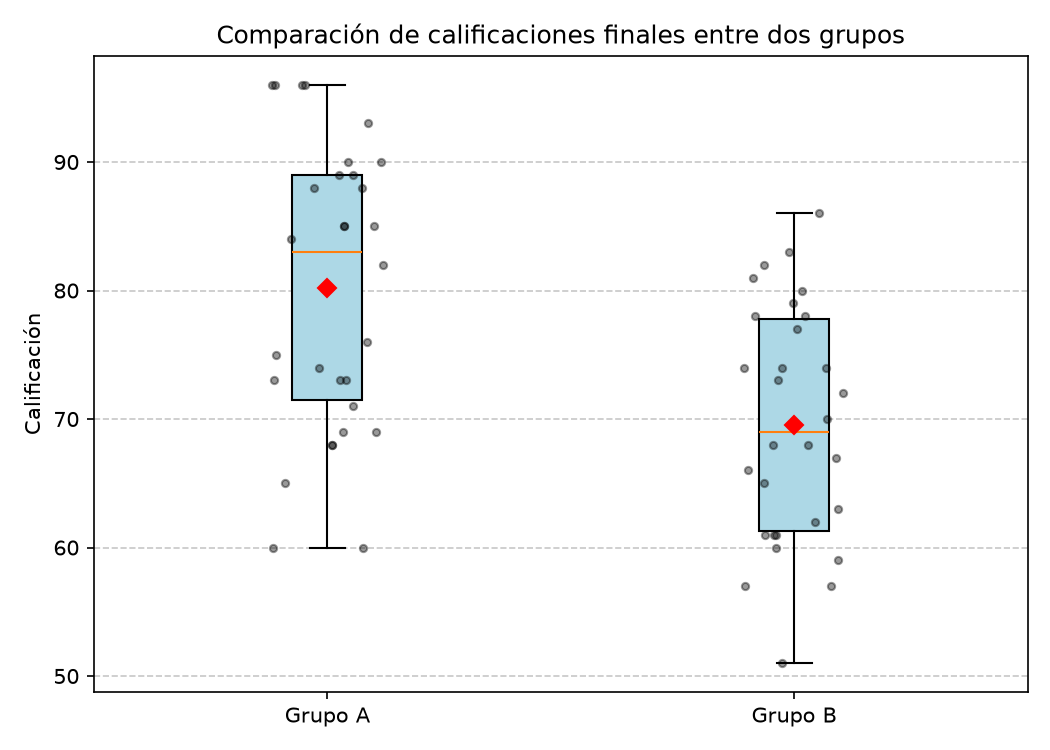
\includegraphics[width=0.72\textwidth]{img/boxplot_ej1.png}
\caption{Diagrama de caja de las calificaciones finales del Grupo A y el Grupo B. El rombo rojo marca la media y los puntos negros, cada estudiante.}
\label{fig:box1}
\end{figure}

\begin{consola}[label=out:box1]{Ejecución de \texttt{act05.py}: Boxplots, Ejercicio 1}
=== Boxplots - Ejercicio 1: calificaciones por grupo ===
             Grupo A  Grupo B
Q1              71.5    61.25
Mediana         83.0    69.00
Q3              89.0    77.75
RIC             17.5    16.50
Bigote inf.     60.0    51.00
Bigote sup.     96.0    86.00
Media           80.2    69.57
Desv. est.      11.2     9.17
Atípicos         0.0     0.00
\end{consola}

\begin{itemize}
    \item \textbf{Mediana.} El Grupo A tiene un desempeño claramente mayor: su mediana es de 83 contra 69 del Grupo B, una diferencia de 14 puntos. Además, la mediana del Grupo A (83) está por encima del tercer cuartil del Grupo B (77.75), lo que significa que más de la mitad del Grupo A supera al 75\,\% de los estudiantes del Grupo B.
    \item \textbf{Dispersión.} Ambos grupos tienen una variabilidad parecida: el RIC es de 17.5 en el Grupo A y de 16.5 en el Grupo B, y las desviaciones estándar son de 11.2 y 9.17. La diferencia entre los grupos está en el nivel de las calificaciones, no en su dispersión.
    \item \textbf{Valores atípicos.} Ningún grupo presenta valores atípicos: los bigotes llegan hasta los valores mínimo y máximo de cada grupo. Esto es esperable, porque el código base simula las calificaciones con una distribución uniforme (\texttt{randint}) acotada entre 60 y 99 para el Grupo A y entre 50 y 94 para el Grupo B, que no genera valores extremos.
    \item \textbf{Forma.} En el Grupo A la media (80.2) es menor que la mediana (83) y la mediana está más cerca de $Q_3$ que de $Q_1$, lo que indica un ligero sesgo a la izquierda: hay más dispersión entre las calificaciones bajas del grupo.
\end{itemize}

\subsection{Boxplots, Ejercicio 2: tiempos de espera en tres sucursales}

\begin{figure}[htbp]
\centering
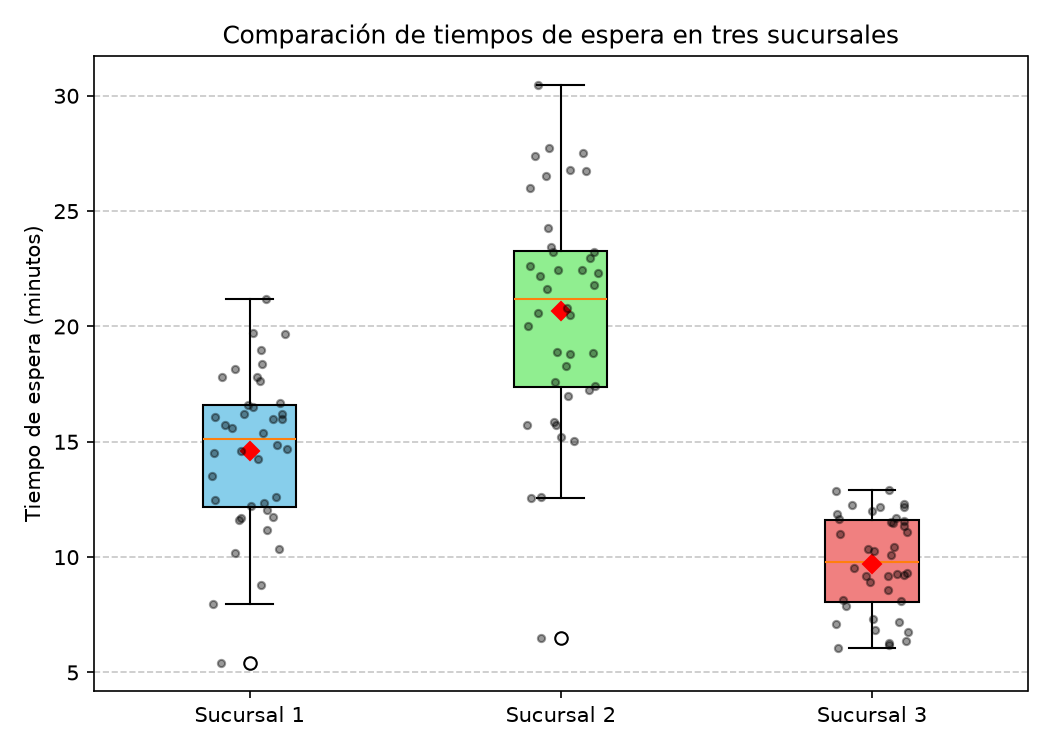
\includegraphics[width=0.72\textwidth]{img/boxplot_ej2.png}
\caption{Diagrama de caja de los tiempos de espera en tres sucursales. Los círculos vacíos son valores atípicos.}
\label{fig:box2}
\end{figure}

\begin{consola}[label=out:box2]{Ejecución de \texttt{act05.py}: Boxplots, Ejercicio 2}
=== Boxplots - Ejercicio 2: tiempos de espera por sucursal ===
             Sucursal 1  Sucursal 2  Sucursal 3
Q1                12.16       17.38        8.05
Mediana           15.13       21.19        9.81
Q3                16.61       23.29       11.60
RIC                4.44        5.91        3.55
Bigote inf.        7.97       12.57        6.08
Bigote sup.       21.18       30.47       12.89
Media             14.58       20.67        9.71
Desv. est.         3.44        4.96        2.13
Atípicos           1.00        1.00        0.00
Valores atípicos en Sucursal 1: [5.43]
Valores atípicos en Sucursal 2: [6.48]
\end{consola}

\begin{itemize}
    \item \textbf{Mediana.} Las tres sucursales tienen niveles de espera muy diferentes. La Sucursal 3 es la más rápida (mediana de 9.81 minutos), la Sucursal 1 es intermedia (15.13) y la Sucursal 2 es la más lenta (21.19). Las cajas de las sucursales 2 y 3 ni siquiera se traslapan.
    \item \textbf{Variabilidad.} La Sucursal 2 es la más variable: tiene el mayor RIC (5.91 minutos), la mayor desviación estándar (4.96) y los bigotes más largos, que van de 12.57 a 30.47 minutos. La Sucursal 3 es la más consistente, con un RIC de 3.55 y una desviación estándar de 2.13. Es decir, en la Sucursal 2 los clientes no solo esperan más, sino que su tiempo de espera es menos predecible.
    \item \textbf{Valores atípicos.} Las sucursales 1 y 2 tienen un valor atípico cada una, ambos por debajo de su bigote inferior: un cliente esperó solo 5.43 minutos en la Sucursal 1 y otro 6.48 minutos en la Sucursal 2. Son tiempos inusualmente cortos para esas sucursales, aunque serían normales en la Sucursal 3. En la práctica conviene revisarlos, porque podrían ser errores de captura o casos especiales, como un cliente con cita previa.
\end{itemize}

\subsection{Histogramas, Ejercicio 1: tiempos de entrega}

\begin{figure}[htbp]
\centering
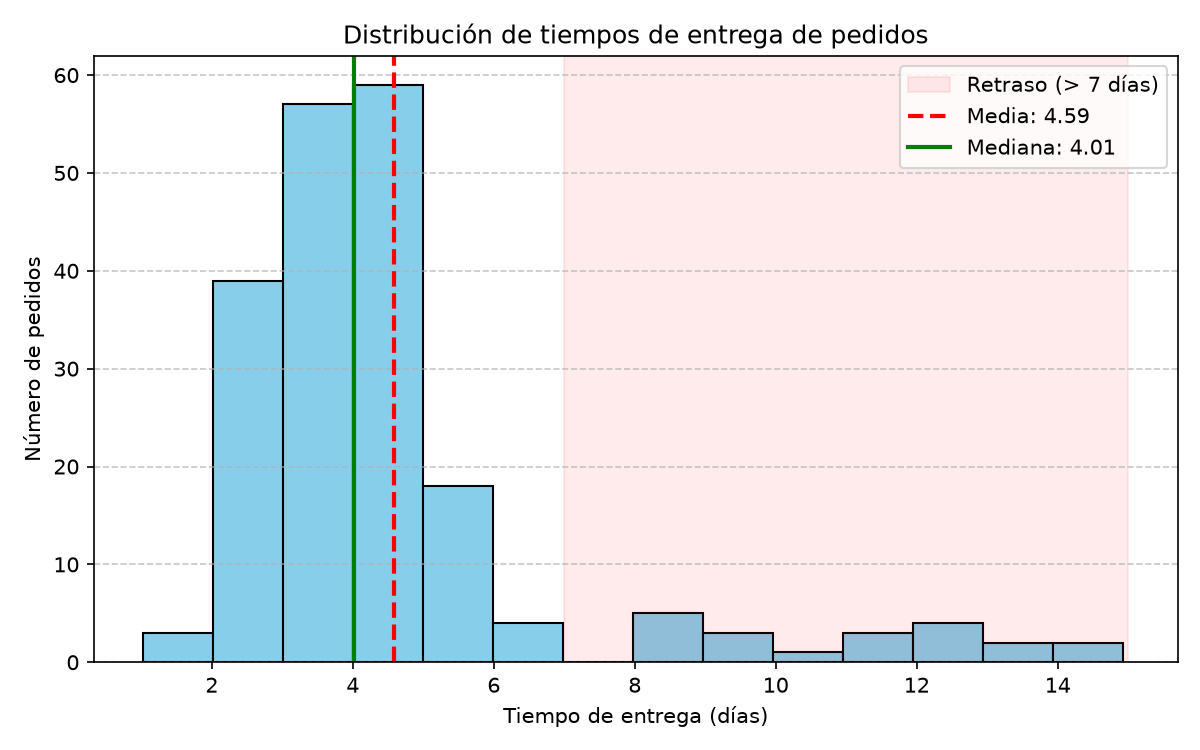
\includegraphics[width=0.78\textwidth]{img/histograma_ej1.png}
\caption{Histograma de los tiempos de entrega de 200 pedidos. La zona sombreada corresponde a entregas de más de 7 días.}
\label{fig:hist1}
\end{figure}

\begin{consola}[label=out:hist1]{Ejecución de \texttt{act05.py}: Histogramas, Ejercicio 1}
=== Histogramas - Ejercicio 1: tiempos de entrega ===
count    200.00
mean       4.59
std        2.47
min        1.03
25%        3.25
50%        4.01
75%        4.82
max       14.93
Mediana: 4.01 días
Pedidos entregados entre 2 y 7 días: 88.5%
Pedidos con más de 7 días: 20 (10.0%)
\end{consola}

\begin{itemize}
    \item \textbf{Forma.} La distribución está sesgada a la derecha: la mayoría de los pedidos forma un pico entre 3 y 5 días y hay una cola larga de entregas tardías que llega hasta casi 15 días. Por eso la media (4.59 días) es mayor que la mediana (4.01 días), como ocurre en toda distribución con sesgo positivo \parencite{tecnm2026_documento_fuente}.
    \item \textbf{Eficiencia.} El proceso logístico funciona bien para la mayoría de los pedidos: el 88.5\,\% se entrega entre 2 y 7 días, y la mitad llega en 4 días o menos. El 50\,\% central de las entregas se concentra en un intervalo estrecho, entre 3.25 y 4.82 días.
    \item \textbf{Retrasos.} El histograma muestra un hueco entre 7 y 8 días, seguido de un grupo separado de 20 pedidos (10\,\%) que tardaron entre 8 y 15 días. Este patrón sugiere que los retrasos no son simplemente la cola de las entregas normales, sino un grupo con una causa distinta, como pedidos sin inventario, envíos a zonas lejanas o incidencias con la paquetería. Para el gerente, esos pedidos son el principal punto de mejora.
\end{itemize}

\subsection{Histogramas, Ejercicio 2: calificaciones del examen}

\begin{figure}[htbp]
\centering
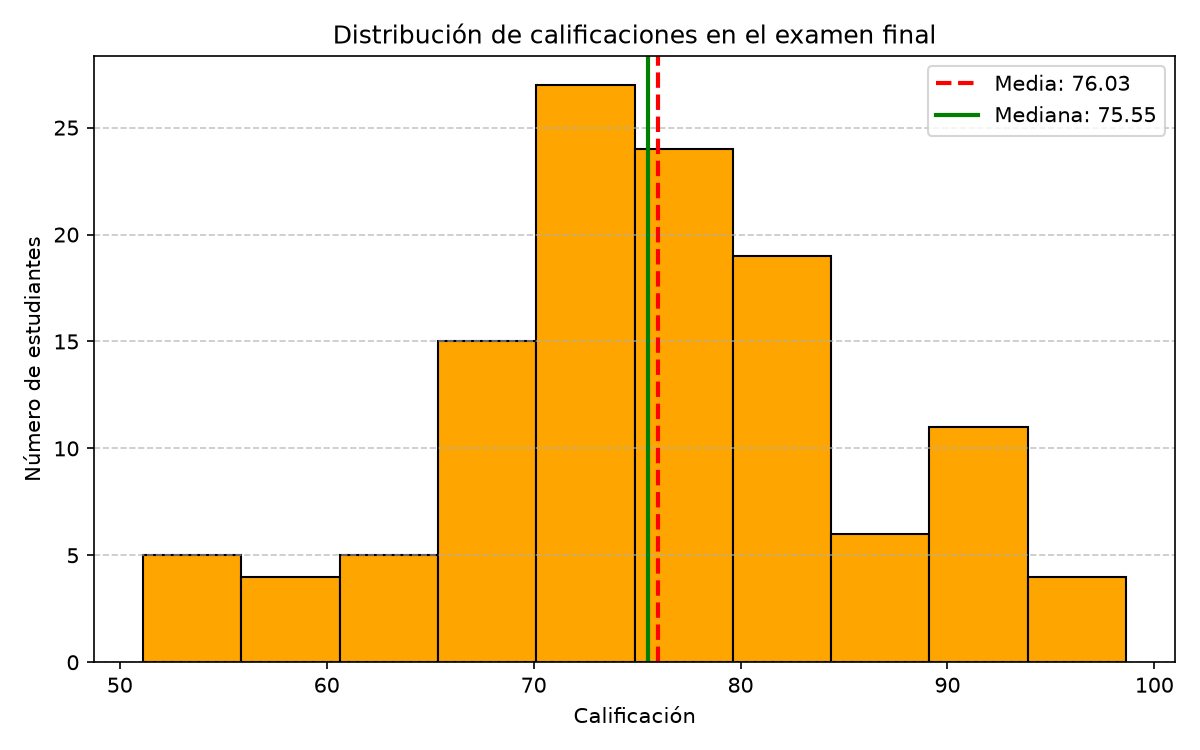
\includegraphics[width=0.78\textwidth]{img/histograma_ej2.png}
\caption{Histograma de las calificaciones de 120 estudiantes en el examen final de matemáticas.}
\label{fig:hist2}
\end{figure}

\begin{consola}[label=out:hist2]{Ejecución de \texttt{act05.py}: Histogramas, Ejercicio 2}
=== Histogramas - Ejercicio 2: calificaciones ===
count    120.00
mean      76.03
std        9.89
min       51.12
25%       70.69
50%       75.55
75%       81.22
max       98.63
Mediana: 75.55
       Estudiantes  Porcentaje
Rango
< 60             8         6.7
60-70           21        17.5
70-80           52        43.3
80-90           26        21.7
> 90            13        10.8
\end{consola}

\begin{itemize}
    \item \textbf{Forma y centro.} La distribución es aproximadamente simétrica y unimodal, con el pico entre 70 y 80. La media (76.03) y la mediana (75.55) casi coinciden, lo que confirma la simetría \parencite{tecnm2026_documento_fuente}.
    \item \textbf{Rango típico.} El 82.5\,\% de los estudiantes obtuvo entre 60 y 90, como indica el enunciado, y el 43.3\,\% se concentra entre 70 y 80. El 50\,\% central de las calificaciones está entre 70.69 y 81.22.
    \item \textbf{Casos excepcionales.} En las colas aparecen 8 estudiantes (6.7\,\%) con menos de 60 y 13 (10.8\,\%) con más de 90. Como los casos muy bajos y muy altos se reparten en ambos extremos, se compensan y no desplazan la media. Para el docente, el grupo con menos de 60 identifica a los estudiantes que podrían necesitar apoyo adicional.
\end{itemize}

\subsection{Dispersión, Ejercicio 1: horas de estudio vs. calificación}

\begin{figure}[htbp]
\centering
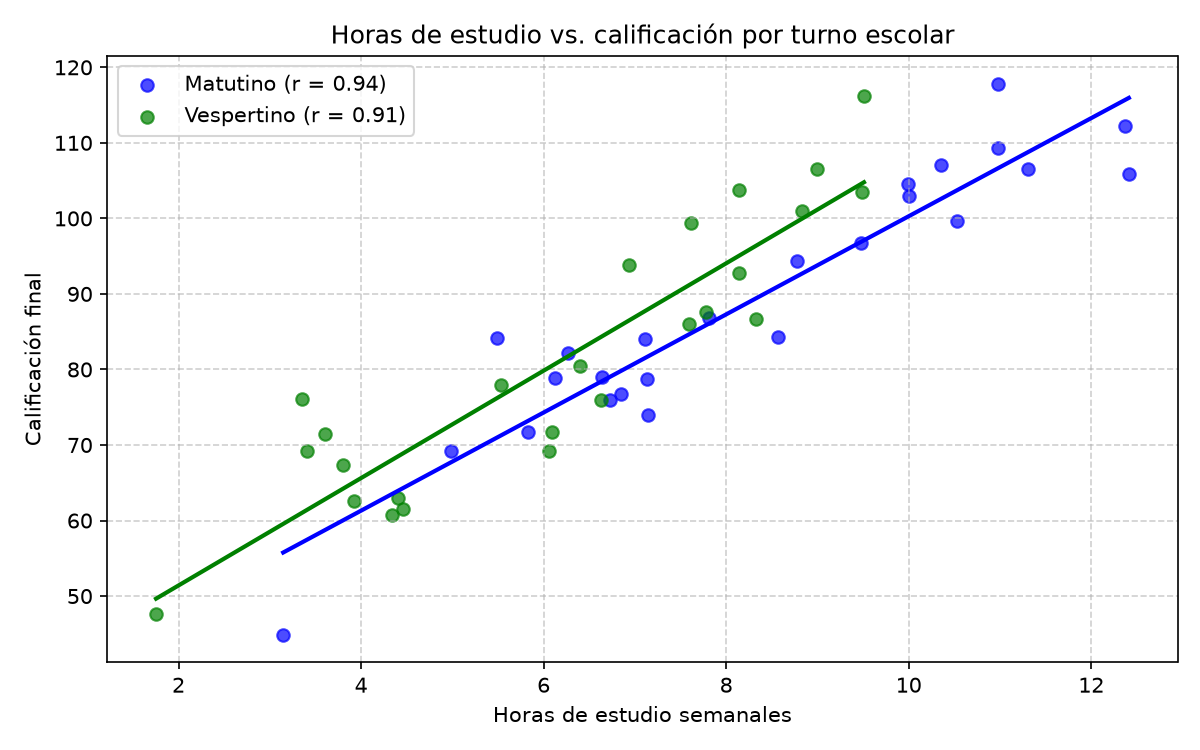
\includegraphics[width=0.78\textwidth]{img/dispersion_ej1.png}
\caption{Diagrama de dispersión entre las horas de estudio semanales y la calificación final, por turno, con la recta de regresión de cada turno.}
\label{fig:disp1}
\end{figure}

\begin{consola}[label=out:disp1]{Ejecución de \texttt{act05.py}: Dispersión, Ejercicio 1}
=== Dispersión - Ejercicio 1: horas de estudio vs. calificación ===
                      Matutino  Vespertino
Horas (media)             8.28        6.20
Calificación (media)     89.11       81.29
Pendiente                 6.50        7.11
Ordenada                 35.32       37.19
r de Pearson              0.94        0.91
Calificaciones mayores a 100 (Matutino): 8
Calificaciones mayores a 100 (Vespertino): 5
\end{consola}

\begin{itemize}
    \item \textbf{Relación entre variables.} En ambos turnos existe una relación lineal positiva y muy fuerte entre las horas de estudio y la calificación, con $r = 0.94$ en el matutino y $r = 0.91$ en el vespertino. Las pendientes indican que cada hora de estudio adicional se asocia con unos 6.5 puntos más en el turno matutino y 7.1 en el vespertino.
    \item \textbf{Diferencia entre turnos.} Los estudiantes del turno matutino estudian en promedio 8.28 horas semanales, contra 6.20 del vespertino, y obtienen una calificación media mayor (89.11 contra 81.29). Sin embargo, las rectas de regresión muestran lo contrario cuando se compara a estudiantes con las mismas horas de estudio: la recta del turno vespertino queda por encima de la del matutino, entre 4 y 8 puntos en el rango de 4 a 10 horas. Es decir, la mayor calificación media del turno matutino se explica porque sus estudiantes estudian más horas, no porque el turno por sí mismo produzca mejores calificaciones.
    \item \textbf{Separabilidad.} Los puntos de ambos turnos se traslapan casi por completo. Desde el punto de vista de la clasificación, las horas de estudio y la calificación no permitirían distinguir a qué turno pertenece un estudiante.
    \item \textbf{Validez de la simulación.} El código base genera la calificación como una función lineal de las horas sin limitarla, por lo que 13 estudiantes (8 del matutino y 5 del vespertino) obtienen calificaciones mayores a 100, que no son posibles en una escala de 0 a 100. En datos reales, valores así indicarían errores de captura que habría que corregir antes del análisis.
\end{itemize}

\subsection{Dispersión, Ejercicio 2: edad vs. colesterol}

\begin{figure}[htbp]
\centering
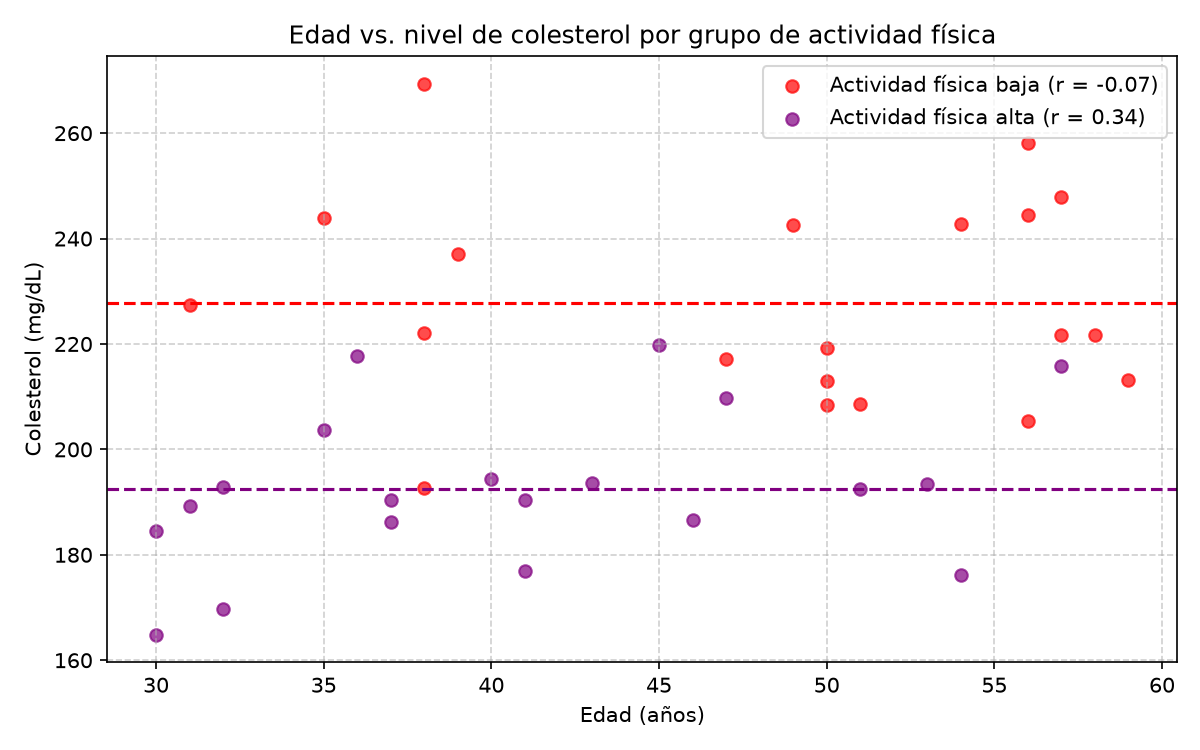
\includegraphics[width=0.78\textwidth]{img/dispersion_ej2.png}
\caption{Diagrama de dispersión entre la edad y el nivel de colesterol, por grupo de actividad física. Las líneas discontinuas marcan el colesterol medio de cada grupo.}
\label{fig:disp2}
\end{figure}

\begin{consola}[label=out:disp2]{Ejecución de \texttt{act05.py}: Dispersión, Ejercicio 2}
=== Dispersión - Ejercicio 2: edad vs. colesterol ===
                         Actividad física baja  Actividad física alta
Edad (media)                             48.45                  40.90
Colesterol (media)                      227.82                 192.44
Colesterol (desv. est.)                  19.64                  15.06
r de Pearson                             -0.07                   0.34
Diferencia de colesterol medio (baja - alta): 35.39 mg/dL

Figuras guardadas en img/
\end{consola}

\begin{itemize}
    \item \textbf{Diferencia entre grupos.} El patrón más claro es la separación vertical entre los grupos. Los pacientes con actividad física baja tienen un colesterol medio de 227.82\,mg/dL, 35.39\,mg/dL más que los de actividad física alta (192.44\,mg/dL). Además, el colesterol es más variable en el grupo de actividad baja (desviación estándar de 19.64 contra 15.06).
    \item \textbf{Relación con la edad.} Dentro de cada grupo no se observa una relación clara entre edad y colesterol: $r = -0.07$ en el grupo de actividad baja y $r = 0.34$, una correlación débil, en el de actividad alta. Esto es consistente con el código base, que simula la edad y el colesterol de forma independiente.
    \item \textbf{Separabilidad.} Los grupos se traslapan entre unos 193 y 220\,mg/dL, pero fuera de esa franja la separación es clara: los 12 pacientes con colesterol mayor a 220\,mg/dL tienen actividad física baja, y ningún paciente de actividad física alta supera ese valor. Por tanto, el nivel de colesterol es una característica útil para distinguir el grupo de actividad física, mientras que la edad aporta poca información adicional.
\end{itemize}

\section{Conclusiones}

Los tres tipos de gráficos ofrecen información complementaria. Los diagramas de caja resumen en un solo gráfico la mediana, la dispersión y los valores atípicos de varios grupos, y facilitan su comparación directa: permitieron ver que el Grupo A supera al Grupo B en nivel pero no en variabilidad, y que la Sucursal 2 es a la vez la más lenta y la menos predecible. Los histogramas, en cambio, revelan la forma de la distribución. En los tiempos de entrega mostraron un sesgo a la derecha y un grupo separado de pedidos retrasados que el diagrama de caja no habría distinguido de una simple cola. Los diagramas de dispersión con un color por clase muestran a la vez la relación entre dos variables y la separación entre grupos.

Las extensiones al código base fueron clave para pasar de la observación visual a conclusiones precisas. Calcular los valores que dibuja cada caja permitió identificar exactamente los valores atípicos. Marcar la media y la mediana en los histogramas hizo evidente el sesgo. Las rectas de regresión y los coeficientes de correlación cuantificaron relaciones que en la gráfica solo se intuyen. Por ejemplo, mostraron que la mayor calificación media del turno matutino se debe a que sus estudiantes estudian más horas, y que la edad no se relaciona con el colesterol.

Desde la perspectiva de la clasificación, estas visualizaciones ayudan a decidir qué características vale la pena usar en un modelo. El nivel de colesterol separa bien los grupos de actividad física, mientras que las horas de estudio no permiten distinguir el turno. Finalmente, el análisis mostró la importancia de revisar críticamente los datos, incluso los simulados: las calificaciones mayores a 100 del primer diagrama de dispersión serían un error a corregir antes de entrenar cualquier modelo.

\referencias

\end{document}
